\newpage
\bignumberedpart{Моделювання}

\subsection{Практичний доказ}
\label{poc}
Для доказу роботи та дослідження роботи алгоритму був написаний прототип (proof of concept) \cite{rader2014cdr}. Алгоритм \ref{alg:general_anomaly_detection} реалізований без змін мовою Python. Візуалізація шаблонів двох класів користувачів на \autoref{fig:model_poc_1}. Перший клас - абоненти, що роблять дзвінки на початку і в кінці робочого дня, а також активні у вихідні дні. Другий клас - типово корпоративні користувачі, що роблять дзвінки в бізнес-години. Як видно, вноситься випадкова складова по днях тижня, і для кожного абонента вона своя.

У імітаторі є можливість провести інтервенцію однієї групи користувачів, або декількох, переводячи з одного сталого стану в інший. Таким чином є можливість протестувати роботу системи виявлення аномальної поведінки.

\begin{figure}[h]
        \begin{center}
            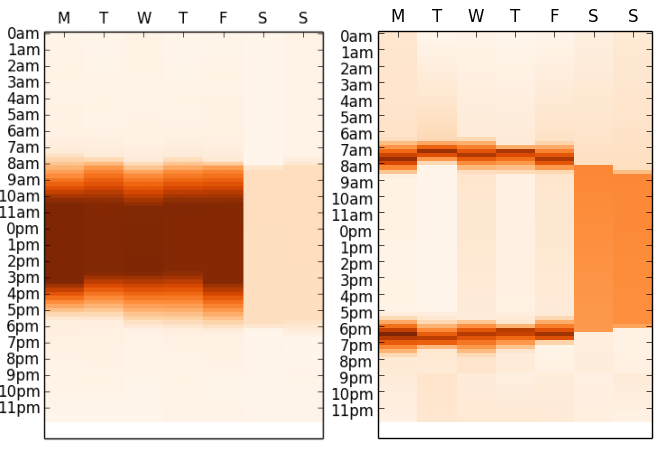
\includegraphics[scale=0.4]{resources/model_1_2.png}
        \end{center}
        \caption{Два класи імітованих абонентів}
        \label{fig:model_poc_1}
\end{figure}

Проаналізовано роботу алгоритму в трьох випадках:
\begin{itemize}
  \item Інтервенція в роботу тільки одного абонента (\autoref{fig:model_poc_one});
  \item Інтервенція в роботу одного класу абонентів, робота без урахування тренда (\autoref{fig:model_poc_group_notrend}). По осі абсцис - час у годинах (в моделі) з початку роботи системи, по осі ординат - кількість дзвінків;
  \item Інтервенція в роботу одного класу абонентів, робота з урахуванням тренда (\autoref{fig:model_poc_group}).
\end{itemize}


\begin{figure}[h!]
        \begin{center}
            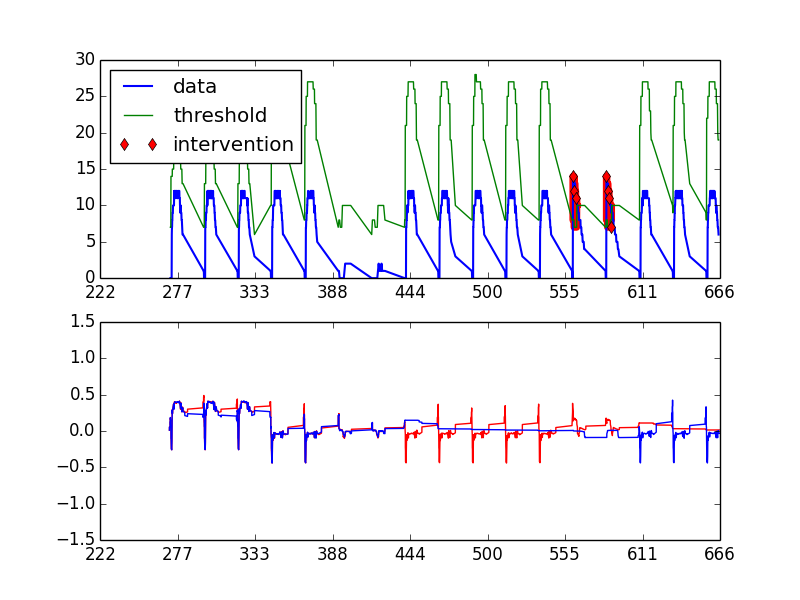
\includegraphics[scale=0.6]{resources/model_1_3_one.png}
        \end{center}
        \caption{Одинична інтервенція одного телефонного номера у вихідні дні. По осі абсцис - час у годинах (в моделі) з початку роботи системи, по осі ординат - кількість дзвінків}
        \label{fig:model_poc_one}
\end{figure}

\begin{figure}[h!]
        \begin{center}
            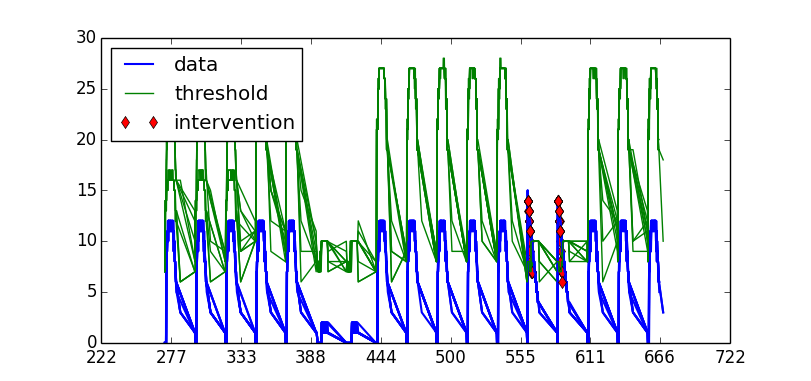
\includegraphics[scale=0.6]{resources/model_1_4_group_notrend.png}
        \end{center}
        \caption{Інтервенція в роботу одного класу абонентів без урахування тренда}
        \label{fig:model_poc_group_notrend}
\end{figure}

\begin{figure}[h!]
        \begin{center}
            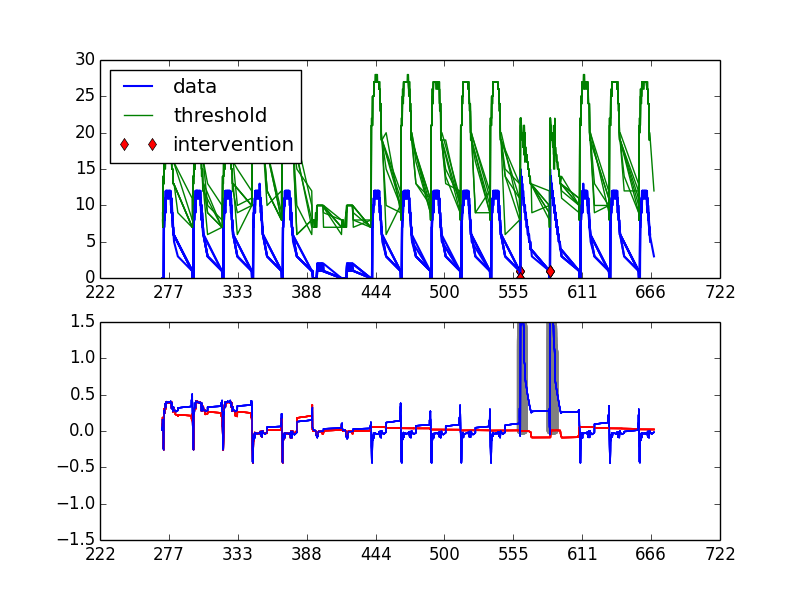
\includegraphics[scale=0.6]{resources/model_1_5_group.png}
        \end{center}
        \caption{Інтервенція в роботу класу абонентів з урахуванням тренда}
        \label{fig:model_poc_group}
\end{figure}


На верхніх графіках показана залежність кількості дзвінків, максимально допустиму кількість дзвінків і точками позначені виявлені інтервенції. На нижніх графіках показаний тренд.

Як видно, при інтервенції в роботу одного абонента (\autoref{fig:model_poc_one}) тренд не змінюється і інтервенція виявляється легко (кількість підозрілих дзвінків практично збігається з фактичною).

При груповій зміні поведінки (\autoref{fig:model_poc_group}) видно два піки лінії тренда, що припадають на вихідні дні (в даному досліді користувачі, які ніколи не дзвонили по вихідних змінюють цю поведінку). На верхньому графіку видно, що рівень інтервенцій дуже низький, що означає правильну роботу алгоритму - групова зміна поведінка не вважається підозрілим.

Для перевірки, другий дослід був проведений з тими ж вихідними даними, але без урахування тренда (\autoref{fig:model_poc_group_notrend}). На графіку видно, що рівень інтервенцій практично збігається з кількістю фактичних дзвінків в даній ділянці, що значить високу ймовірність шахрайства. Таким чином, спосіб обліку групових змін дійсно зменшує кількість помилкових спрацьовувань.

Як видно з \autoref{fig:model_poc_time}, час обробки одного запису не є константним. Ця характеристика стає гіршою із збільшенням кількості абонентів.

\begin{figure}[h!]
        \begin{center}
            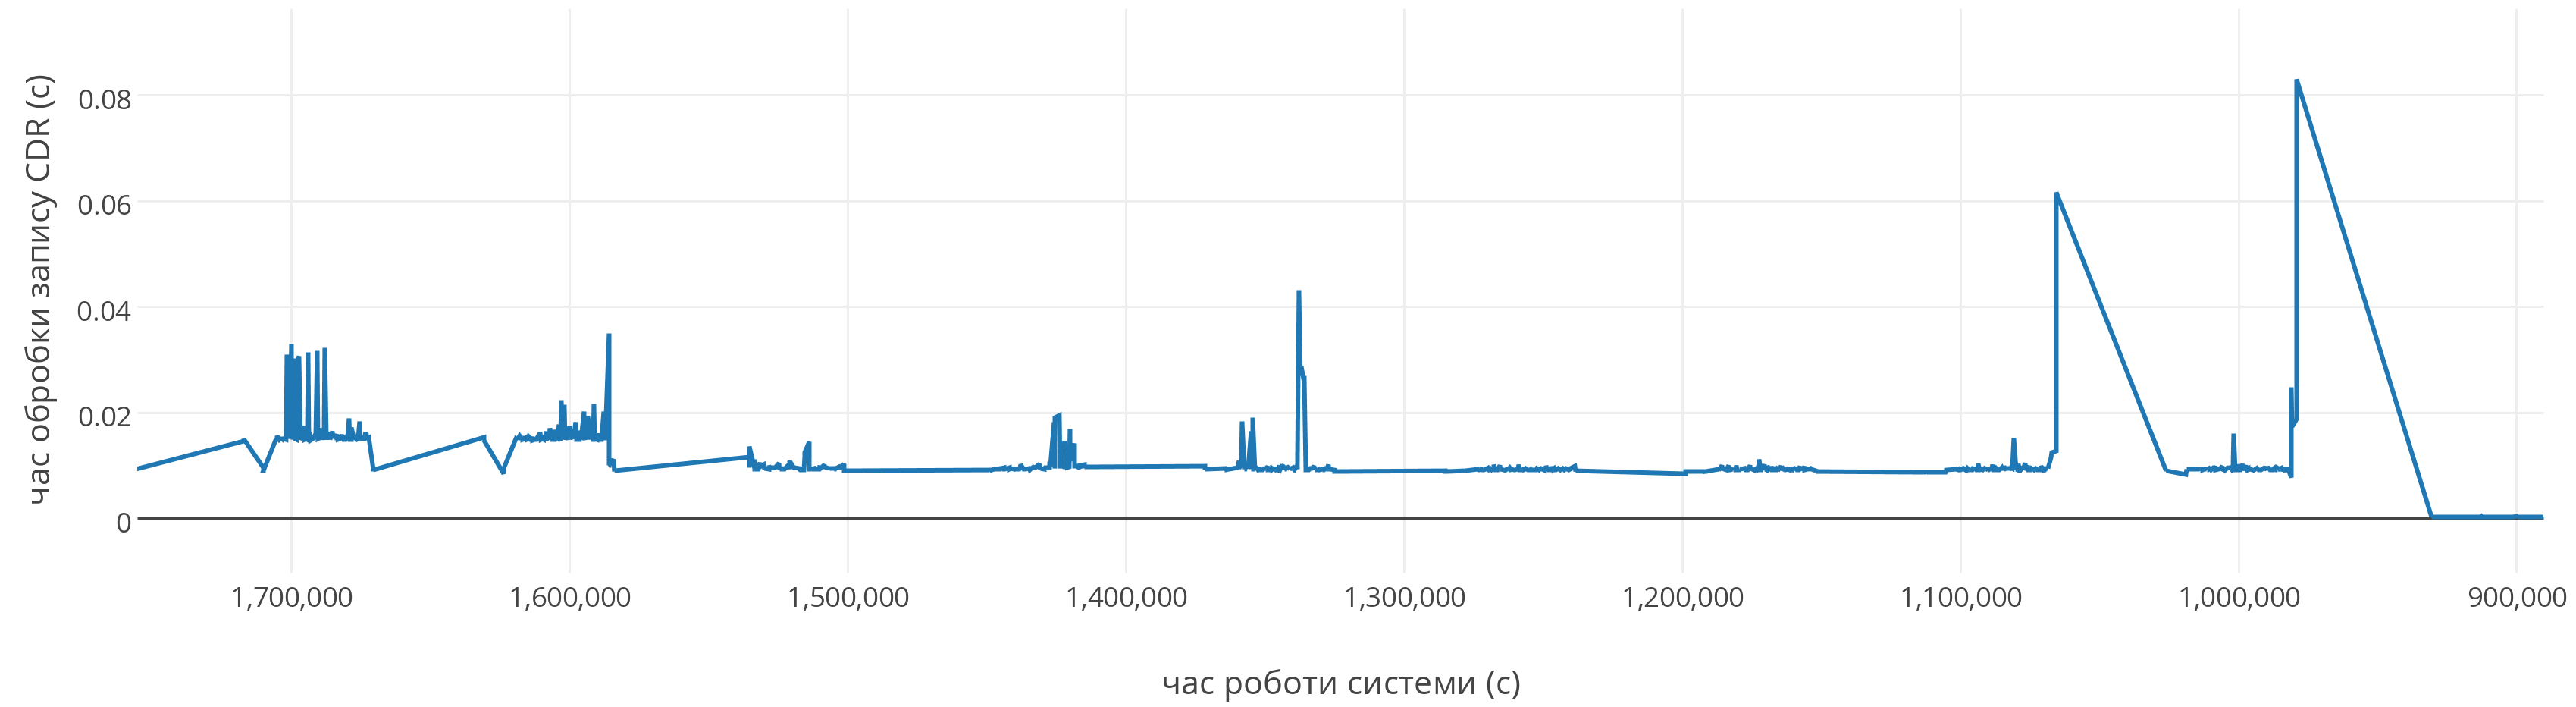
\includegraphics[scale=0.13]{resources/poc-time.png}
        \end{center}
        \caption{Час обробки записів у прототипі системи}
        \label{fig:model_poc_time}
\end{figure}

\subsection{Реалізація алгоритму після модифікації}

Для усунення недоліків вихідного алгоритму, він був декомпозований для роботи в паралельному режимі (розділ \ref{parallel}).

Імітатор налаштований для роботи з двома класами абонентів (\autoref{fig:model_prod_1}).

\begin{figure}[h!]
        \begin{center}
            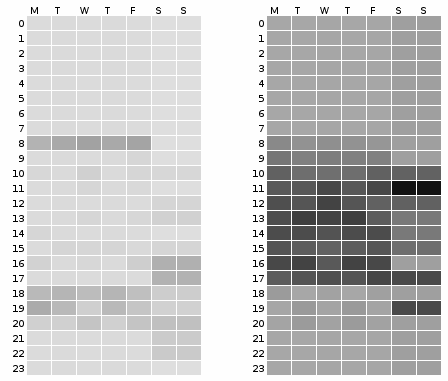
\includegraphics[scale=0.6]{resources/model_2_1.png}
        \end{center}
        \caption{Два класи імітованих абонентів}
        \label{fig:model_prod_1}
\end{figure}

В результаті класифікації кожен абонент потрапляє в одну з k груп (На \autoref{fig:model_prod_2} позначені кольорами та цифрою зверху справа).

\begin{figure}[h!]
        \begin{center}
            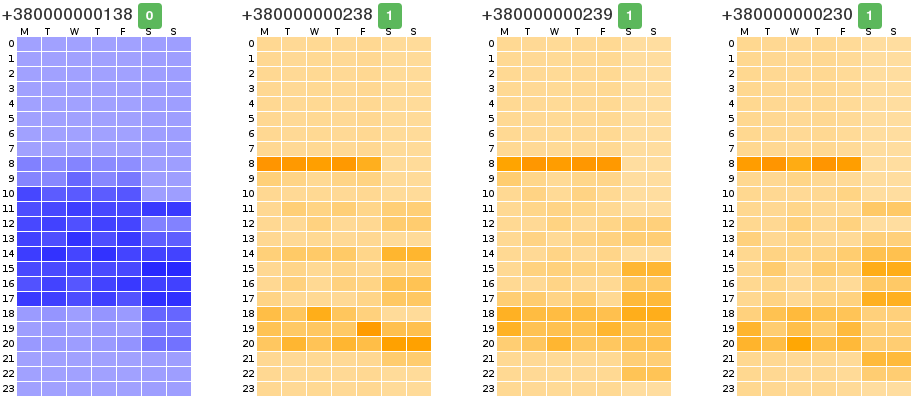
\includegraphics[scale=0.4]{resources/model_2_2.png}
        \end{center}
        \caption{Результат класифікації абонентів}
        \label{fig:model_prod_2}
\end{figure}

Як видно з порівняння \autoref{fig:model_prod_time} та \autoref{fig:model_poc_time}, у розробленій системі враховані недоліки першої реалізації, час обробки одного запису зменшився на 50\%, при чому в новій реалізації характеристика не залежить від кількості абонентів чи класів.

\begin{figure}[h!]
        \begin{center}
            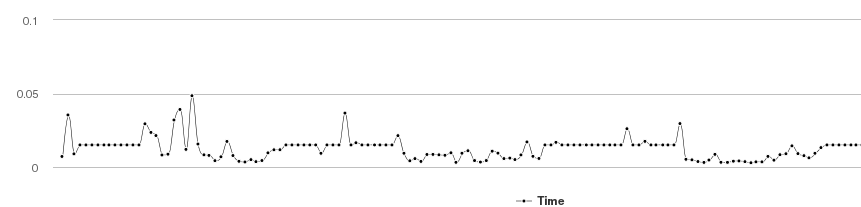
\includegraphics[scale=0.5]{resources/system-time.png}
        \end{center}
        \caption{Час обробки записів у розробленій системи}
        \label{fig:model_prod_time}
\end{figure}

\subsection{Робота системи в реальному часі}

Дана система може працювати в режимі реального часу, тому що модифікований алгоритм дає константний час обробки одного запису.

Як було зазначено, в даному способі місцем, що обмежує паралелизм є точка підрахунку тренду, в якій потрібно обмінюватись поточними частотами із всіма нодами через загальну пам'ять. В реалізованій системі роль загальної пам'яті грає мережеве сховище Redis типу ключ-значення. Враховуючи спосіб підрахунку тренду, запис поточної частоти в сховище можна робити кожну кратну кількість опрацьованих записів, таким чином обмежуючи канал з базою даних. Сховище Redis легко маштабується на читання, тому враховуючи вищесказане, алгоритм може маштабуватися лінійно.

На комп'ютері, на якому проводилося моделювання це значення приблизно дорівнює $T_1 = 0.01$ с. В виробничій системі це значення буде меншим, тому що нода, яка відповідає за підрахунки буди окремим комп'ютером, не суміщеним із імітатором абонентів, але збільшиться час на передачу даних по мережі. Така система здатна обробляти до $6000$ записів за хвилину, або $100$ за секунду.

За офіційними результатами досліджень швидкості роботи черги Apache Kafka, вона може передавати у систему до $50$ МБ/с, що складає $250000$ повідомлень в секунду на один брокер, за умови що одне повідомлення складає $200$ байт. За офіційними результатами досліджень швидкості роботи Apache Storm, він може обробляти до $1000000$ записів в секунду на одній ноді. Виходячи з цього, Kafka є більш повільною системою, тому що працює із диском та реплікує дані для відмовостійкості.

\begin{table}[h]
    \caption{Кількість оброблених записів в секунду в залежності від швидкості обробки на одному вузлі та кількості вузлів}
    \begin{tabularx}{\textwidth}{| X | X | X | X | X | X |}
        \hline
        $T_1$  & 1     & 2    & 5     & 10    & 50     \\ \hline
        0.01   & 100   & 200  & 500   & 1000  & 5000 \\ \hline
        0.005  & 200   & 400  & 1000  & 2000  & 10000 \\ \hline
        0.001  & 1000  & 2000 & 5000  & 10000 & 50000 \\ \hline
        0.0005 & 2000  & 4000 & 10000 & 20000 & 100000 \\ \hline
        0.0001 & 10000 & 20000 & 50000 & 100000 & 500000 \\ \hline
    \end{tabularx}
    \label{tab:realtime-calculate}
\end{table}

Отже, згідно з розрахунками \autoref{tab:realtime-calculate} для досягнення теоретичного максимуму в 250000 повідомлень в секунду на одному брокері, потрібно мати кластер Storm, що складається із 25 вузлів та може обробляти один запис за $T_1 = 0.0001$ c, або 50 вузлів та швидкістю в $T_1 = 0.0002$. Пропускна здатність кластеру такого розміру при $T_1 = 0.01$ буде $N=\frac{1}{0.01} \cdot 50 = 5000$ записів CDR в секунду.

Пропускна здатність мережі в випадку з теоретичним максимумом має складати $M = 50 \cdot 8 = 400$ Мбіт без сигнального трафіку, що можна забеспечити із мережею швидкістю в 1 Гбіт.

\subsection{Моделювання за відсутності інтервенцій}

Після моделювання 100 абонентів, по 50 абонентів на один шаблон поведінки, отримані такі дані. На \autoref{fig:model_prod_3} зображено графік аналізу одного із абонентів мережі. Як видно з графіку, реальне використання абонентом мережі (суцільна лінія) близька до розрахованого шаблону поведінки (пунктирна лінія), та лежить в межах довірчого інтервалу 95\% (сіра зона на графіку).

\begin{figure}[h!]
        \begin{center}
            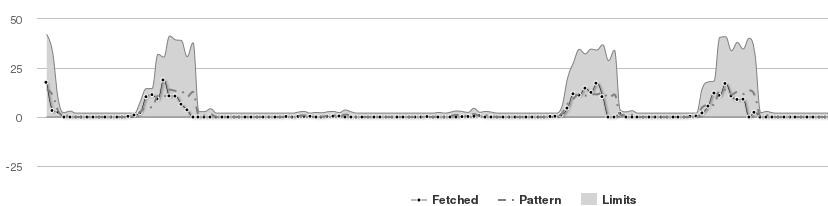
\includegraphics[scale=0.55]{resources/model_2_3.png}
        \end{center}
        \caption{Графік аналізу роботи одного з абонентів}
        \label{fig:model_prod_3}
\end{figure}

Відхилення частоти використання мережі абоненту від шаблонної (\autoref{fig:model_prod_4}) в межах допустимих границь.

\begin{figure}[h!]
        \begin{center}
            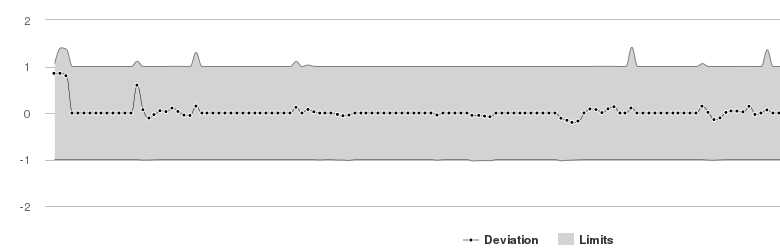
\includegraphics[scale=0.55]{resources/model_2_4.png}
        \end{center}
        \caption{Графік відхилення частоти дзвінків одного з абонентів від шаблону}
        \label{fig:model_prod_4}
\end{figure}

За відсутності змін поведінки, тренд (\autoref{fig:model_prod_5}) флуктує біля позначки 0.

\begin{figure}[h!]
        \begin{center}
            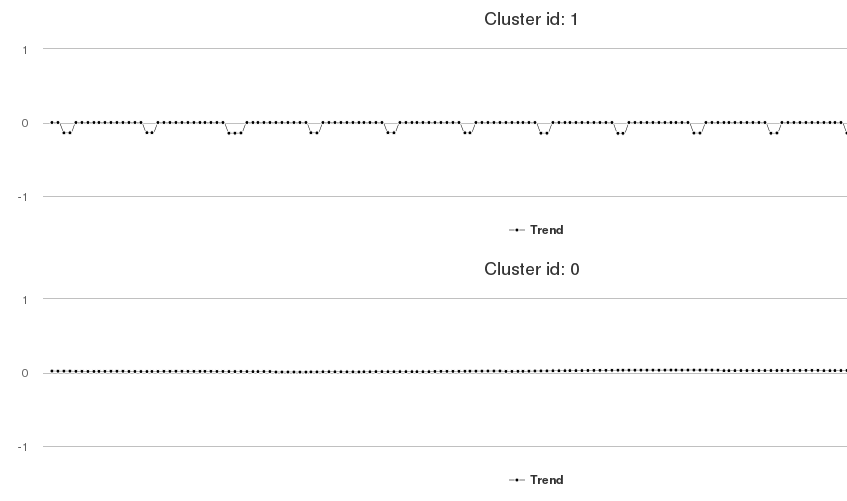
\includegraphics[scale=0.55]{resources/model_2_5.png}
        \end{center}
        \caption{Графік тренду, розрахованого для двох кластерів}
        \label{fig:model_prod_5}
\end{figure}

\subsection{Моделювання інтервенції в роботу одного абонента без урахування тренду}

\begin{figure}[h!]
        \begin{center}
            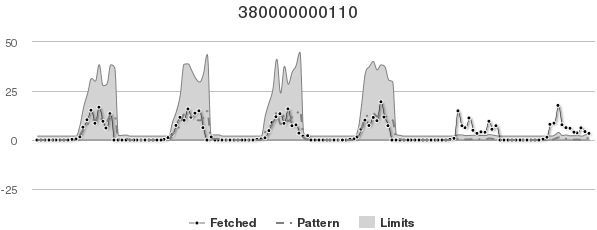
\includegraphics[scale=0.55]{resources/oneIntervWithoutTrend/analysis.png}
        \end{center}
        \caption{Графік аналізу роботи абоненту, який змінює поведінку}
        \label{fig:model_oneIntervWithoutTrend_analysis_int}
\end{figure}
На \autoref{fig:model_oneIntervWithoutTrend_analysis_int} та \autoref{fig:model_oneIntervWithoutTrend_dev_int} зображено графіки використання мережі та відхилень від шаблонної поведінки. Як видно з першого графіку, зміна поведінки є виходом частоти використання мережі за довірчі інтервали. З другого графіку видно, що система успішно визначила аномалії.

В даному випадку групових змін в поведінці не було, та розрахунок та врахування тренду (врахування групових змін в поведінці) було відімкнуто.

\begin{figure}[h!]
        \begin{center}
            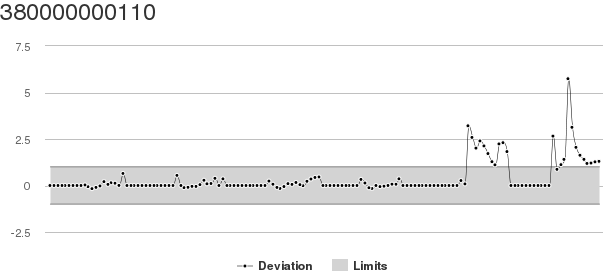
\includegraphics[scale=0.55]{resources/oneIntervWithoutTrend/dev.png}
        \end{center}
        \caption{Графік відхилення від шаблону абоненту, який змінює поведінку}
        \label{fig:model_oneIntervWithoutTrend_dev_int}
\end{figure}

\label{oneIntervWithoutTrend}

\subsection{Моделювання інтервенції в роботу одного абонента з урахуванням тренду}
\begin{figure}[h!]
        \begin{center}
            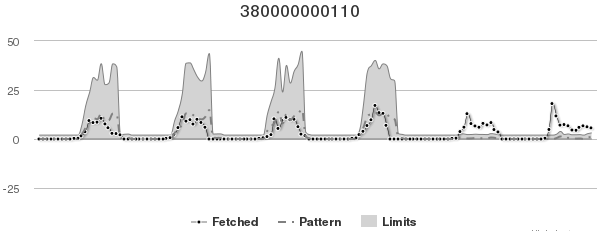
\includegraphics[scale=0.55]{resources/oneIntervWithTrend/analysis-int.png}
        \end{center}
        \caption{Графік аналізу роботи абоненту, який змінює поведінку}
        \label{fig:model_oneIntervWithTrend_analysis_int}
\end{figure}

\begin{figure}[h!]
        \begin{center}
            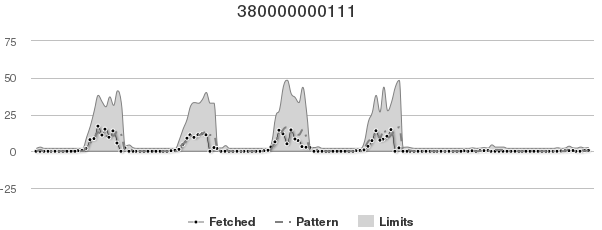
\includegraphics[scale=0.55]{resources/oneIntervWithTrend/analysis-ok.png}
        \end{center}
        \caption{Графік аналізу роботи абоненту, який не змінює поведінку}
        \label{fig:model_oneIntervWithTrend_analysis_ok}
\end{figure}
На \autoref{fig:model_oneIntervWithTrend_analysis_int} та \autoref{fig:model_oneIntervWithTrend_analysis_ok} зображено графіки використання мережі двох абонентів, один змінює поведінку, другий - ні відповідно. Зміну поведінки видно із виходу рівня використання мережі за довірчі інтервали на першому графіку.

\begin{figure}[h!]
        \begin{center}
            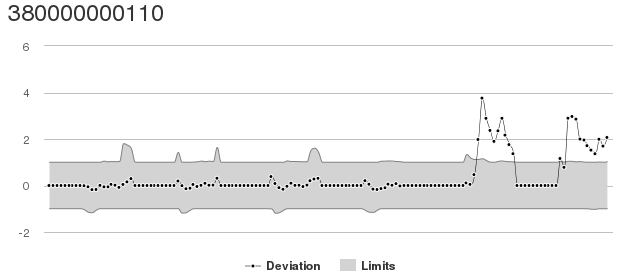
\includegraphics[scale=0.55]{resources/oneIntervWithTrend/dev-int.png}
        \end{center}
        \caption{Графік відхилення від шаблону абоненту, який змінює поведінку}
        \label{fig:model_oneIntervWithTrend_dev_int}
\end{figure}

\begin{figure}[h!]
        \begin{center}
            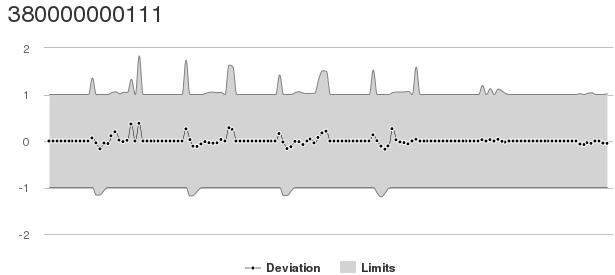
\includegraphics[scale=0.55]{resources/oneIntervWithTrend/dev-ok.png}
        \end{center}
        \caption{Графік відхилення від шаблону абоненту, який не змінює поведінку}
        \label{fig:model_oneIntervWithTrend_dev_ok}
\end{figure}

З \autoref{fig:model_oneIntervWithTrend_dev_int} видно, що система успішно виявила інтервенцію (відхилення від нормальної поведінки вийшло за довірчий інтервал). При цьому, ця зміна не впливає аналіз поведінки інших користувачів через тренд (\autoref{fig:model_oneIntervWithTrend_dev_ok}).

\begin{figure}[h!]
        \begin{center}
            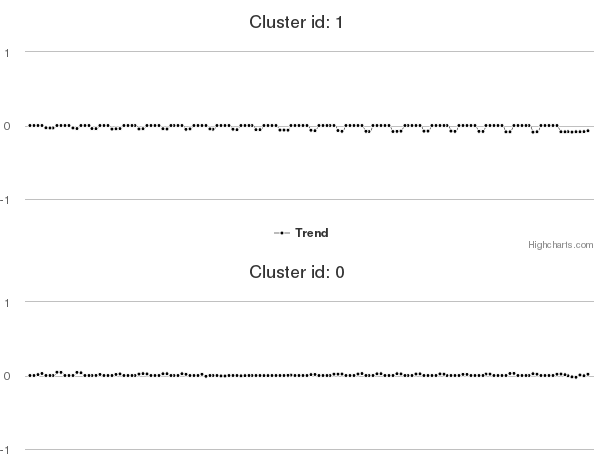
\includegraphics[scale=0.55]{resources/oneIntervWithTrend/trend.png}
        \end{center}
        \caption{Графіки трендів для двох класів абонентів}
        \label{fig:model_oneIntervWithTrend_trend}
\end{figure}

В даному випадку групових змін в поведінці не було, але розрахунок та врахування тренду (врахування групових змін в поведінці) було ввімкнено.

Співставляючи результати моделювання без урахування тренду (розділ \ref{oneIntervWithoutTrend}) та з урахуванням тренду, бачимо що врахування групової поведінки не заважає виявленню одиночних інтервенцій. Зміна роботи одного з користувачів не впливає на загальний тренд всього кластеру (\autoref{fig:model_oneIntervWithTrend_trend}).

\subsection{Моделювання інтервенції у клас абонентів без урахування тренду}
\label{classWithoutTrend}
В даному випадку зміна шаблону використання системи відбулася одночасно у цілого класу користувачів. Врахування групової поведінки (тренду) відімкнено.

\begin{figure}[h!]
        \begin{center}
            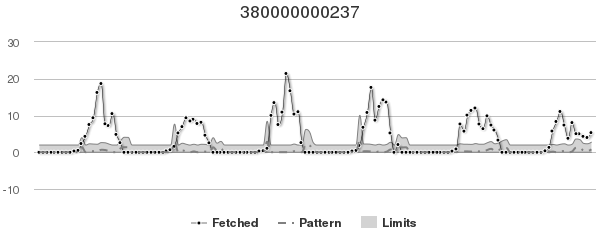
\includegraphics[scale=0.55]{resources/classIntervWithoutTrend/analysis.png}
        \end{center}
        \caption{Графік аналізу роботи одного з абонентів, що змінили поведінку}
        \label{fig:model_classIntervWithoutTrend_analytics}
\end{figure}

\begin{figure}[h!]
        \begin{center}
            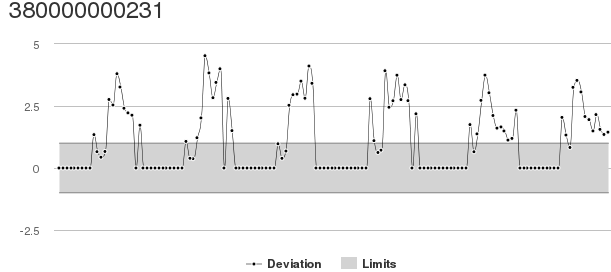
\includegraphics[scale=0.55]{resources/classIntervWithoutTrend/dev.png}
        \end{center}
        \caption{Графік відхилення від шаблону одного з абонентів, що змінили поведінку}
        \label{fig:model_classIntervWithoutTrend_dev}
\end{figure}

На \ref{fig:model_classIntervWithoutTrend_analytics} та \ref{fig:model_classIntervWithoutTrend_dev} видно, що система помилково визначила поведінку як аномальну, хоча зміна пройшла у всіх абонентів. Таким чином, оператори могли отримати велику кількість хибнопозитивних повідомлень про вторгнення.

\subsection{Моделювання інтервенції у клас абонентів з урахуванням тренду}

В даному випадку зміна шаблону використання системи відбулася одночасно у цілого класу користувачів. Врахування групової поведінки (тренду) ввімкнено.

\begin{figure}[h!]
        \begin{center}
            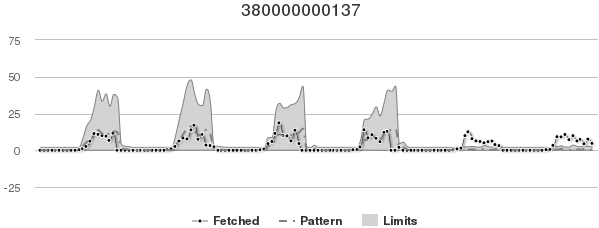
\includegraphics[scale=0.55]{resources/classIntervWithTrend/analysis.png}
        \end{center}
        \caption{Графік аналізу роботи одного з абонентів, що змінили поведінку}
        \label{fig:model_classIntervWithTrend_analytics}
\end{figure}

\begin{figure}[h!]
        \begin{center}
            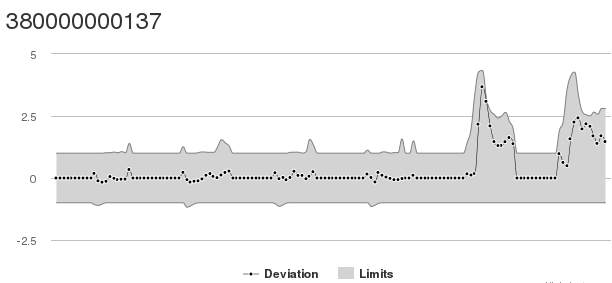
\includegraphics[scale=0.55]{resources/classIntervWithTrend/dev.png}
        \end{center}
        \caption{Графік відхилення від шаблону одного з абонентів, що змінили поведінку}
        \label{fig:model_classIntervWithTrend_dev}
\end{figure}

Як видно з \autoref{fig:model_classIntervWithTrend_analytics} та \autoref{fig:model_classIntervWithTrend_dev}, на відміну від з моделюванням з відімкненим врахуванням групової поведінки (розділ \ref{classWithoutTrend}), поведінка користувачів з групи, що змінила поведінку не була відмічена як аномальне, що каже про правильну роботу алгоритму, який враховує тренд (\autoref{fig:model_classIntervWithTrend_trend}) - характер зміни поведінки групи користувачів.

\begin{figure}[h!]
        \begin{center}
            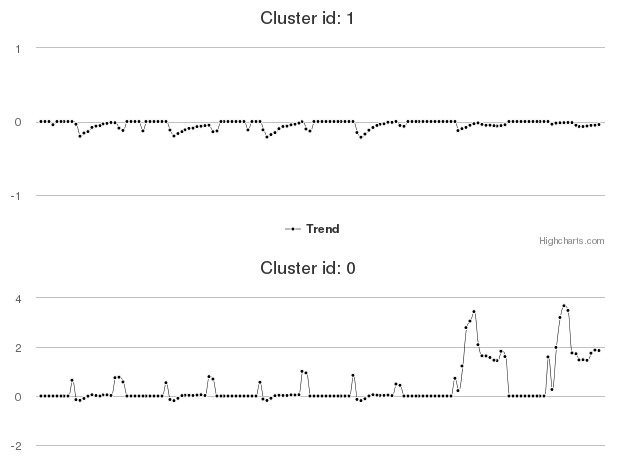
\includegraphics[scale=0.55]{resources/classIntervWithTrend/trend.png}
        \end{center}
        \caption{Графіки трендів для двох класів абонентів}
        \label{fig:model_classIntervWithTrend_trend}
\end{figure}

\clearpage
\subsection*{Висновки до розділу 3}
\addcontentsline{toc}{subsection}{Висновки до розділу 3}

Було промодельовано розроблений прототип системи виявлення аномалій поведінки абонентів телефонної мережі. На базі моделювання були виявлені недоліки та розроблені вимоги до системи. Промодельовано роботу розробленої системи та зроблено порівняння із прототипом.

Проаналізовано роботу алгоритму в багатокористувацькому режимі з урахуванням тренда, а також проведено порівняння з однокористувацьким режимом і багатокористувацьким режимом без урахування тренда режимах для оцінки ефективності методу.

Як видно з результатів моделювання, розроблена система, на відміну від її прототипу, видає константний час на перевірку одного номеру, що дозволяє використовувати систему із обмеженнями реального часу.
